\documentclass[a4paper,german,12pt,smallheadings]{scrartcl}
\usepackage[T1]{fontenc}
\usepackage[utf8]{inputenc}
\usepackage{babel}
\usepackage{tikz}
\usepackage{pgfplots}
\usepackage{geometry}
\usepackage[fleqn]{amsmath}
\usepackage{amssymb}
\usepackage{float}
\usepackage{enumerate}
\usepackage{commath} % http://tex.stackexchange.com/questions/14821/whats-the-proper-way-to-typeset-a-differential-operator
\usepackage{cancel}

% Number only referenced equations
\usepackage[fleqn]{mathtools}
\mathtoolsset{showonlyrefs}

%\usepackage{wrapfig}
\usepackage[thinspace,thinqspace,squaren,textstyle]{SIunits}

% New command for color underlining
\usepackage{xcolor}

\newsavebox\MBox
\newcommand\colul[2][red]{{\sbox\MBox{$#2$}%
  \rlap{\usebox\MBox}\color{#1}\rule[-1.2\dp\MBox]{\wd\MBox}{0.5pt}}}

\restylefloat{table}
\geometry{a4paper, top=15mm, left=10mm, right=20mm, bottom=20mm, headsep=10mm, footskip=12mm}
\linespread{1.5}
\setlength\parindent{0pt}
\DeclareMathOperator{\Tr}{Tr}
\DeclareMathOperator{\Var}{Var}
\begin{document}
\allowdisplaybreaks % Seitenumbrüche in Formeln erlauben
\begin{center}
\bfseries % Fettdruck einschalten
\sffamily % Serifenlose Schrift
\vspace{-40pt}
Atom- und Molekülphysik, Sommersemester 2014, Aufgabenblatt 1

Markus Fenske, Luis Herrmann, Tutor: Michael Kleinert
\vspace{-10pt}
\end{center}
\section*{Aufgabe 1: Potentialtopf I}

Die Herleitung der Energien und der Wellenfunktion sparen wir uns an dieser
Stelle, das war letztes Semester.

\begin{enumerate}[a)]
  \item
    Die Übergangsenergie ist $E_2 - E_1 = \frac{3 \hbar^2 \pi^2}{2 m_e L^2}$.
    Für $L = 1 \; \nano\meter$ ergibt sich eine Energie von $752 \;
    \milli\electronvolt$, für $L = 1 \; \centi\meter$ entsprechend $7{,}52 \cdot
    10^{-15} \;\electronvolt$.
  \item
    Wir nehmen an, dass mit ``mittlere Hälfte'' das Intervall $[\frac{1}{4} L,
    \frac{3}{4} L]$ gemeint ist. Die Aufenthaltswahrscheinlichkeit ist dann
    \begin{align}
        &\int\limits_{\frac{1}{4} L}^{\frac{3}{4} L} \dif x\; \envert{\psi(x)}^2
      =  \frac{2}{L} \int\limits_{\frac{1}{4} L}^{\frac{3}{4} L} \dif x\; \sin^2 \frac{\pi x}{L}
      =  \frac{1}{L} \int\limits_{\frac{1}{4} L}^{\frac{3}{4} L} \dif x\; 1 - \cos \frac{2 \pi x}{L}
      =  \frac{1}{L} \del{ \frac{L}{2} - \sbr{\frac{L}{2 \pi} \sin \frac{2 \pi x}{L}}_{\frac{L}{4}}^{\frac{3L}{4}} } \\
      = \;&\frac{1}{L} \del{\frac{L}{2} + \frac{L}{\pi}}
      = \frac{\pi + 2}{2 \pi}
      \approx 81{,}83 \; \%
    \end{align}
  \item
    Die Funktion mit einem Maximum einspricht $n=1$, die mit zwei Maxima $n=2$, usw.

    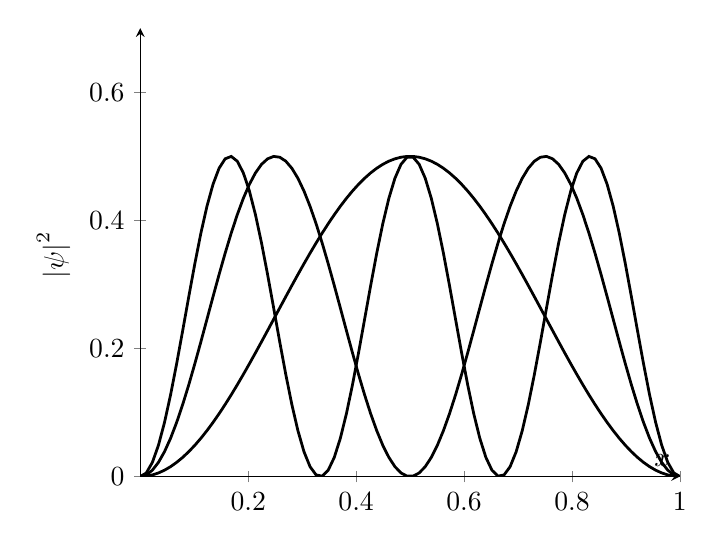
\begin{tikzpicture}
    \begin{axis}
        [% options
        xlabel=$x$,
        ylabel={$\envert{\psi}^2$},
        axis x line = middle,
        axis y line = left,
        xmin=0,
        xmax=1,
        ymin=0,
        ymax=0.7,
        ]
    \addplot[
        domain=0:1,
        samples=90,
        line width = 1pt,
        ]
        {1/2*sin(1*deg(x)*pi)^2};
    \addplot[
        domain=0:1,
        samples=90,
        line width = 1pt,
        ]
        {1/2*sin(2*deg(x)*pi)^2};
    \addplot[
        domain=0:1,
        samples=90,
        line width = 1pt,
        ]
        {1/2*sin(3*deg(x)*pi)^2};
    \end{axis}
    \end{tikzpicture}
\end{enumerate}

\section*{Aufgabe 2: Potentialtopf II}

Die Energie des Photons ist $E = \frac{hc}{\lambda}$, die Übergangsenergie ist
$E_{12} - E_{11} = \frac{23}{2} \frac{\hbar^2 \pi^2}{2 m_e L^2}$ (wobei die 23
von $12^2 - 11^2$ kommt). Durch Gleichsetzen und Umstellen ergibt sich
\begin{align}
  L = \sqrt{\frac{23}{2} \frac{\lambda}{hc} \frac{\hbar^2 \pi^2}{2 m_e}} \approx 1{,}18 \; \nano\meter
\end{align}

Einen Literaturwert konnten wir nicht finden, allerdings scheint der Wert
zumindest in der korrekten Größenordnung zu liegen. $\beta$-Karotin hat in der
Hauptkette 10 Einfachbindungen und 9 Doppelbindungen bei jeweils $154 \;
\pico\meter$ bzw. $134 \; \pico\meter$ Länge, wobei die Struktur nicht linear,
sondern gewinkelt ist. Damit könnten sich Längen in der Größenordnung 1-3
\nano\meter \;ergeben.

\section*{Aufgabe 4: Wasserstoffatom}
\begin{enumerate}[a)]
  \item
    Der Radialteil ist bekannt als $R_{1,0}(r) = 2 \del{
    \frac{1}{a}}^\frac{3}{2} e^{-\frac{r}{a}}$ und $R_{2,0}(r) = \frac{1}{2\sqrt{2}} \del{
    \frac{1}{a}}^\frac{3}{2} \del{2 - \frac{r}{a}} e^{-\frac{r}{a}}$, wobei $a
    \approx a_0 = \frac{4 \pi \epsilon_0 \hbar^2}{m e^2}$ (Bohrscher
    Atomradius $\approx 52{,}9 \pico\meter$).

    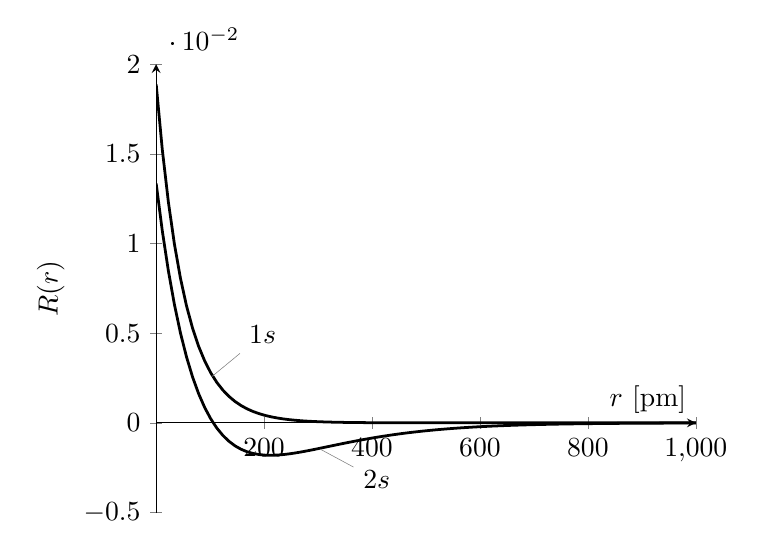
\begin{tikzpicture}
    \begin{axis}
        [% options
        xlabel=$r \text{ [pm]}$,
        ylabel={$R(r)$},
        axis x line = middle,
        axis y line = left,
        xmin=0,
        xmax=1000,
        ymin=-0.005,
        ymax=0.02,
        ]
    \addplot[
        domain=0.1:1000,
        samples=90,
        line width = 1pt,
        ]
        {2*(1/52.9)^(3/2)*exp(-x/52.9)*1/0.274981};
    \addplot[
        domain=0.1:1000,
        samples=90,
        line width = 1pt,
        ]
        {1/2*sqrt(2)*(1/52.9)^(3/2)*(2-x/52.9)*exp(-x/(2*52.9))*1/0.274981};
        \node at (axis cs:300,-0.0014) [pin={340:$2s$},inner sep=0pt] {};
        \node at (axis cs:100,0.0025) [pin={40:$1s$},inner sep=0pt] {};
    \end{axis}
    \end{tikzpicture}
\end{enumerate}
\end{document}
